\section{Introduction}
	The goal of this assignment was to develop a volume renderer based on a raycasting approach. 
	The teacher provided skeleton code with a set-up of the whole graphics pipeline, a reader for volumetric data,
	and a slice-based renderer. The main task was to extend this skeleton code to a full-fledged raycaster. 
	To make such a full-fledged raycaster, we had to implement multiple methods. The first one is the maximum intensity projection.
	Maximum intensity projection takes the highest voxel value along the viewing ray for each pixel.
	We will discuss how we implemented the maximum intensity projection and how we made it faster in Section~\ref{Sec:Mip}. 
	The next method we were asked to implement was the composite transfer function. 
	The composite transfer function performs compositing of colors and opacities of all voxels along the view ray.
	We will discuss the composite transfer function and how we implemented that function in Section~\ref{Sec:Ctf}.
	The last method we were asked to implement was the gradient-based opacity weighting.
	We will describe gradient-based opacity weighting and how we implemented it in Section~\ref{Sec:Gow}.
	After that we will compare all methods and describe these results in Section~\ref{Sec:Com}.
	At last we will describe in Section~\ref{Sec:Con} our conclusions about the methods and their differences.
	
	\begin{figure}[H]
		\centering
		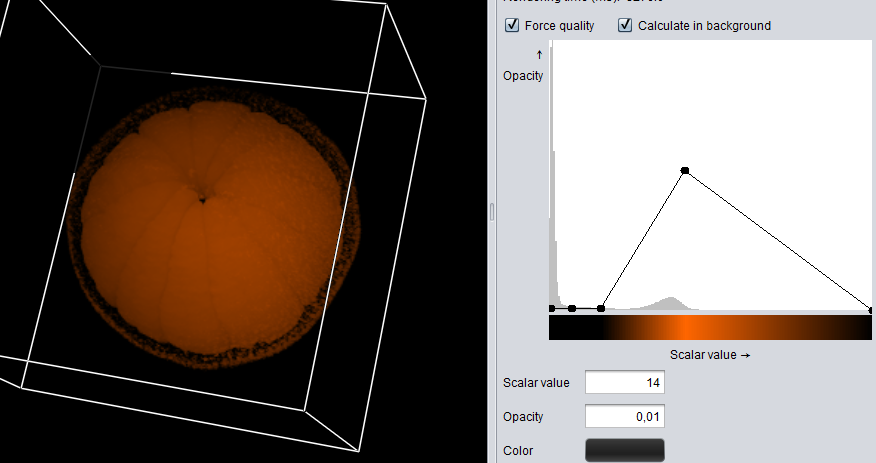
\includegraphics[width=\textwidth]{{img/intro_app}}
		\caption{Overview of our application, showing the orange.fld file rendered with the Composite Transfer Function}
		\label{fig:intro}
	\end{figure}

	Figure~\ref{fig:intro} shows our application running in a browser.
